\documentclass[fleqn,a4paper,12pt]{article}
\usepackage[top=1in, bottom=1in, left=1in, right=1in]{geometry}



\title{Machine Learning Homework 6}
\date{}

\setcounter{section}{0}

\usepackage{listings}

\usepackage{amsmath}
\usepackage{amssymb}


\usepackage{mathspec}
\setmainfont{Noto Serif CJK TC}
% \setmathsfont(Digits,Latin,Greek)[Numbers={Lining,Proportional}]{DejaVu Math TeX Gyre}
\newfontfamily\ZhFont{Noto Serif CJK TC}
\newfontfamily\SmallFont[Scale=0.8]{Droid Sans}
% \newfontfamily\SmallSmallFont[Scale=0.7]{Noto Serif CJK}
\usepackage{fancyhdr}
\usepackage{lastpage}
\pagestyle{fancy}
\fancyhf{}
\rhead{B03902072\ZhFont{江廷睿}}
\lhead{Machine Learning Homework 6}
\rfoot{\thepage / \pageref{LastPage}}

\XeTeXlinebreaklocale "zh"
\XeTeXlinebreakskip = 0pt plus 1pt
\usepackage{parskip}

\usepackage{graphicx}
\usepackage{caption}
\usepackage{subcaption}
\usepackage{float}

\begin{document}
% \maketitle
\thispagestyle{fancy}

\section{(1\%)請比較有無normalize(rating)的差別。並說明如何normalize.}

如果沒有做 normalization,在 valid 上的 RMSE 為 0.862039 ,有做 normalization 則為 0.860133。結論是有沒有做 normalization 沒有太大的差異。normalization 的方式為算出所有評價的平均值與標準差,再將所有評價都減去平均值並除以標準差。

\section{(1\%)比較不同的latent dimension的結果。}

\begin{tabular}[c]{| l | c | r |}
  \hline
  維度 & RMSE \\ \hline
  100 & 0.890224 \\ \hline
  75 & 0.862039 \\ \hline
  50 & 0.877154 \\ \hline
\end{tabular}

這顯示了 latent dimension 並不是愈大愈好,也不是愈小愈好。

\section{(1\%)比較有無bias的結果}

有加入 bias 的 RMSE 是 0.862039 ,沒加 RMSE 則是 bias 0.885437。顯示加入 bias 的確能增進準確度。

\section{(1\%)請試著用DNN來解決這個問題,並且說明實做的方法(方法不限)。並比較MF和NN的結果,討論結果的差異。}

如果訓練時把電影跟使用者的 embedding matrix 接起來,而不是內積,並在後面接上三層的完全連接層,最後輸出層則是一個神經元,則此架構可以到 RMSE 0.877838。相較於加入 bias 後的矩陣分解,效果比較差,但又比不加 bias 的矩陣分解好。 MF 加上 bias 的效果會比較好可能是因為 MF 的假設,也就是用使用者 feature 與電影 feature 的相似度作為評分,可能是有點道理的,所以當這個 domain knowledge 加入後會使得成效較好。但若是資料量夠大,或許 NN 可以做的比 MF 好。

\section{(1\%)請試著將movie的embedding用tsne降維後,將movie category當作label來作圖。}

\begin{figure}[H]
\centering
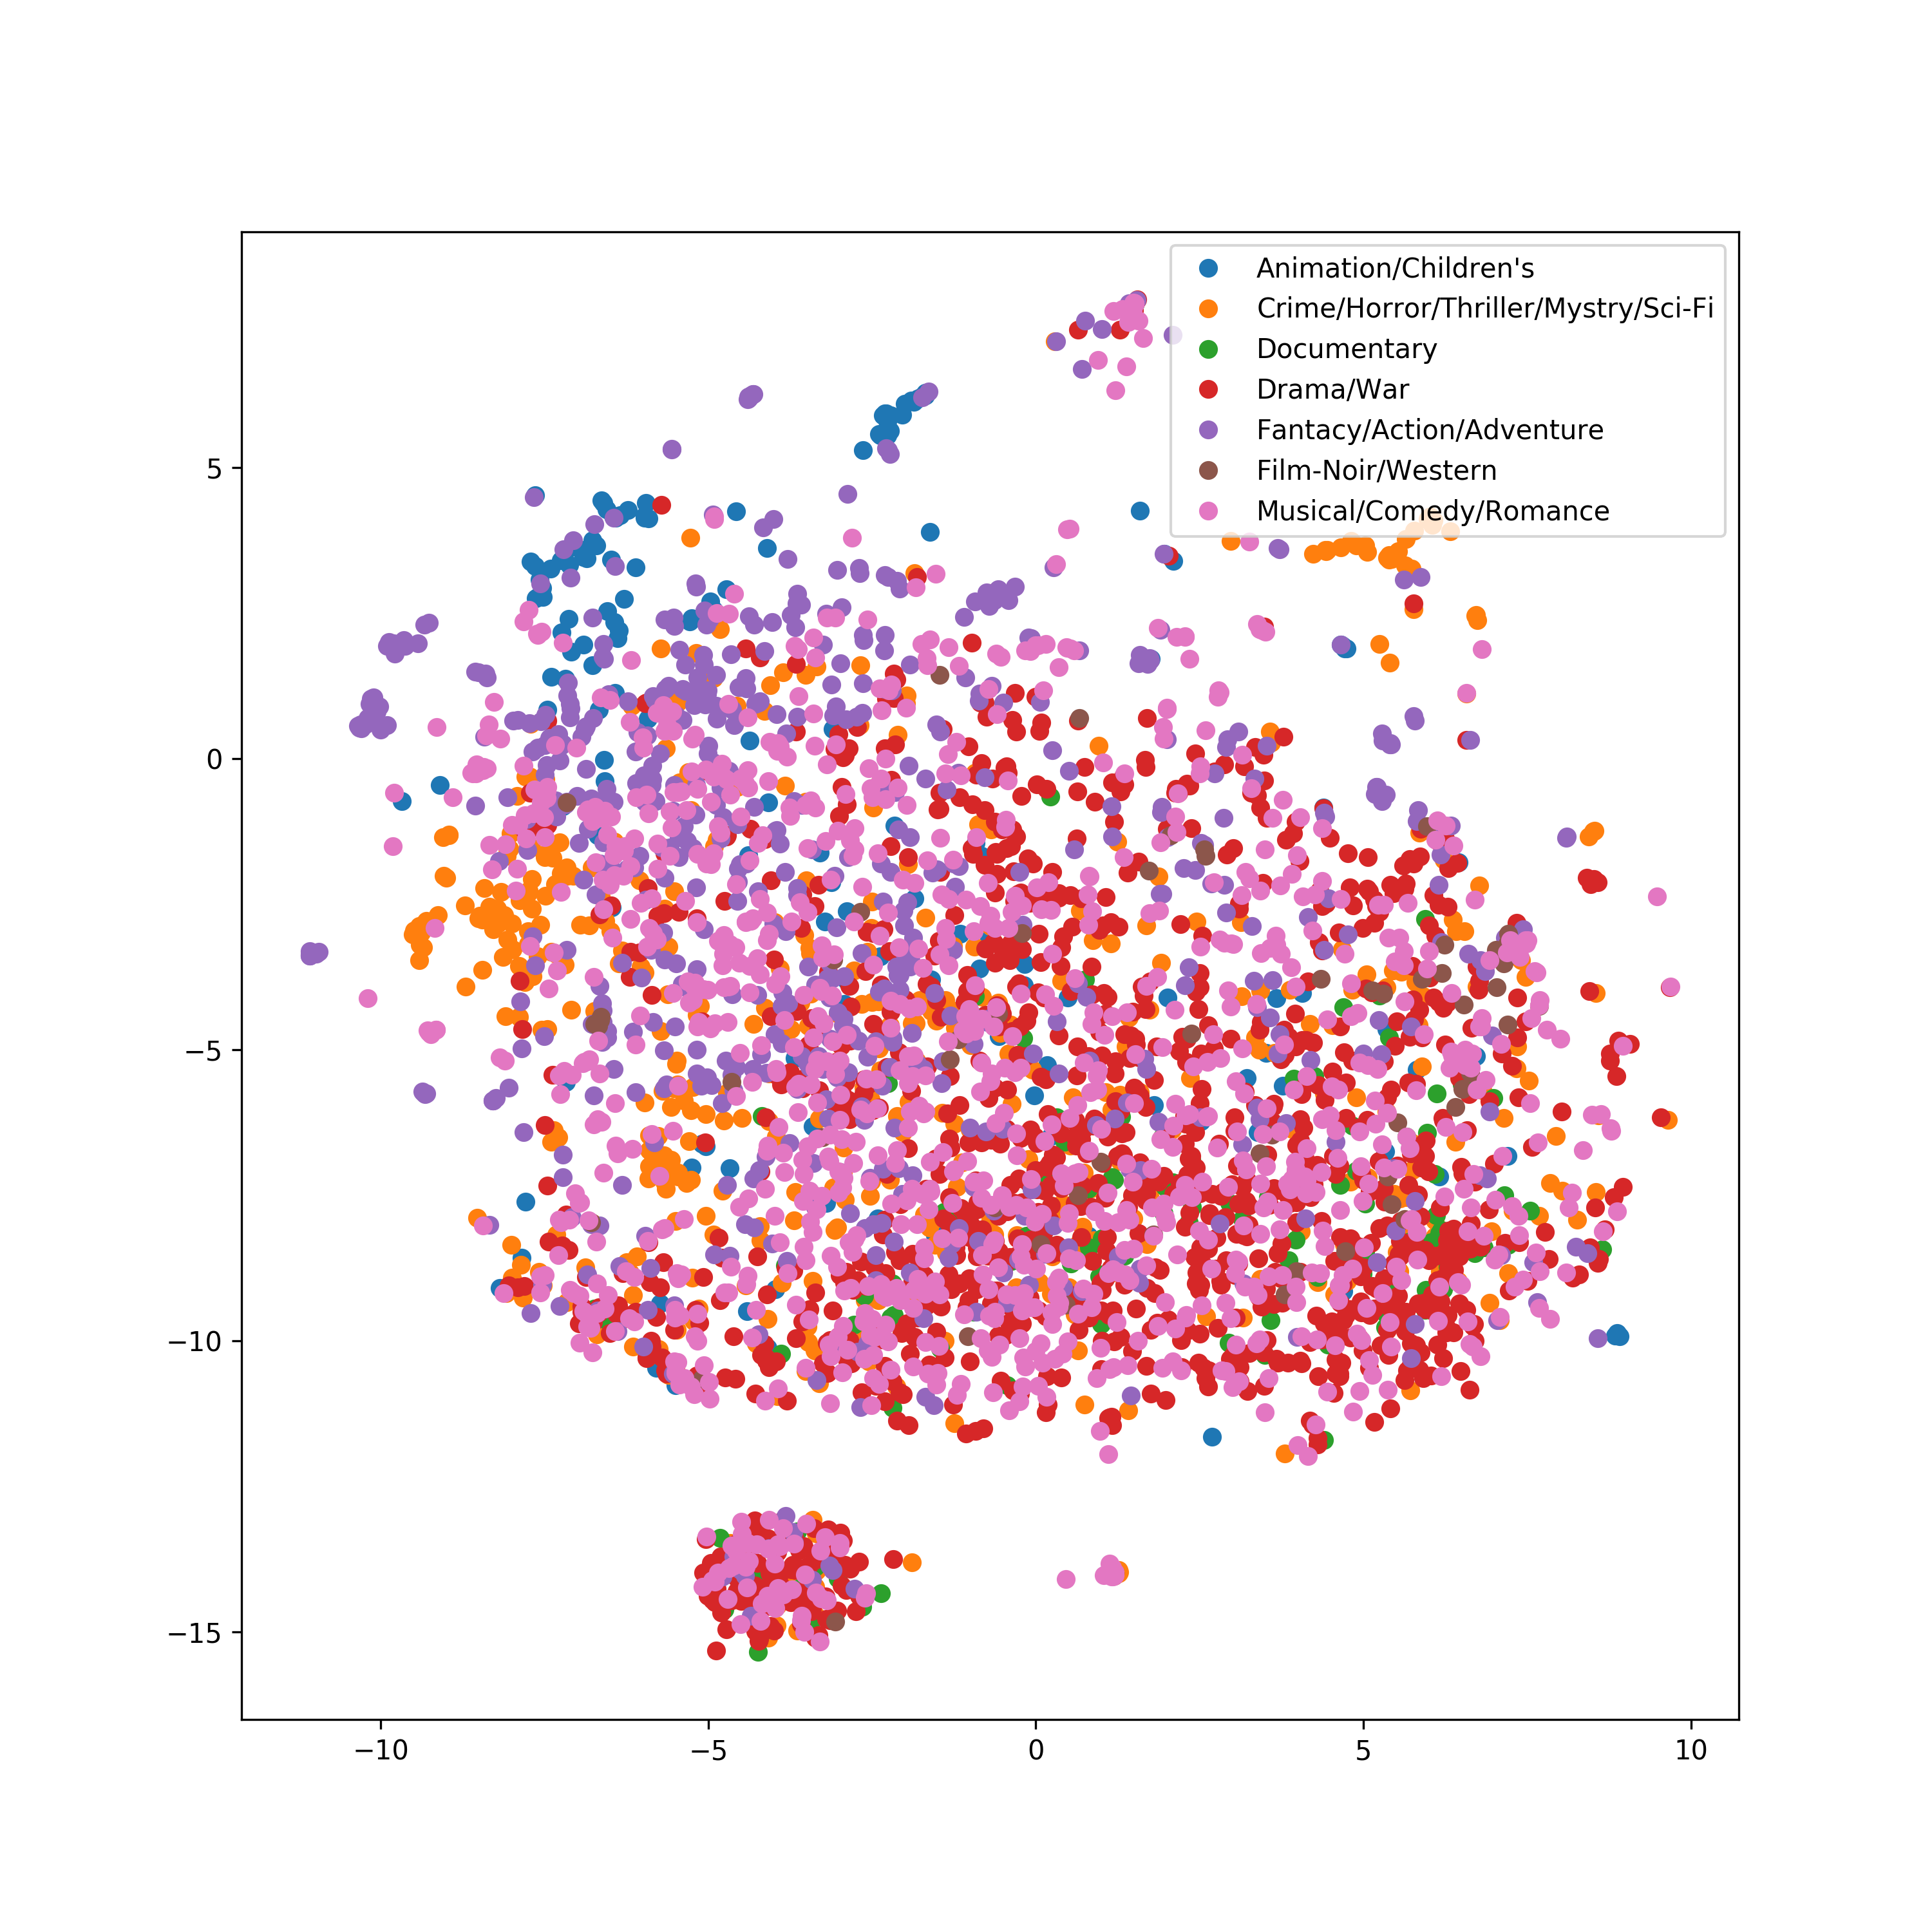
\includegraphics[width=\linewidth]{tsne.png}
\label{fig:p1.1}
\end{figure}

在圖中可以看到, 在圖的左邊 Crime/Horror/Thriller/Mystery/Sci-Fi 有一區較明顯的聚集,而 Animation/Children's 在左上也有一區聚集。顯示學到的 embedding 是有點意義的。

\section{(BONUS)(1\%)試著使用除了rating以外的feature, 並說明你的作法和結果,結果好壞不會影響評分。}

之後又額外增加了使用者的年齡以及電影的年份與類型作為額外的 feature。作法為將使用者與電影額外的 feature 作為不可訓練的 embedding matrix ,分別接在原先矩陣分解的使用者 embedding 與電影的 embedding 之後,讓使用者與電影分別經過一層神經層之後內積作為輸出的預測。最後的 RMSE 為 0.8593 ,稍微比沒有加入額外 features 時好。

\end{document}
